\documentclass[letterpaper, 10pt]{article}

\usepackage[english]{custompack}
\usepackage{fullpage}
\usepackage{amssymb}
\usepackage{multicol}
\usepackage{mathtools}
%\usepackage{hyperref}
%\usepackage{abcproblem}
%\renewcommand{\thesubsection}{\alph{subsection}}

%\allowdisplaybreaks
%\numberwithin{theorem}{section}

\title{\textbf{Assignment 2}}
\author{Håkon Mork \\ ECSE 526 Artificial Intelligence}
\date{February 28, 2013}

\begin{document}
\maketitle
\noindent
\begin{multicols*}{2}

\section{Two-dimensional navigation}
\subsection{State utilities and optimal policy}
% (fold)
After 42 rounds of value iteration, the values converged to:
\[
	\begin{array}{|c|c|c|c|}
		\hline
		0.078 & 0.027 &       & -0.187 \\
		\hline
		0.169 & 0.084 & 0.102 & -0.154 \\
		\hline
		0.283 &       & 0.257 & -1 \\
		\hline
		0.392 & 0.549 & 0.699 & 1 \\
		\hline
	\end{array}
\]
After 6 iterations, the optimal policy converged to:
\[
	\begin{array}{|c|c|c|c|}
		\hline
		\rightarrow & \downarrow &       & \leftarrow \\
		\hline
		\downarrow & \rightarrow & \downarrow & \uparrow \\
		\hline
		\downarrow &       & \downarrow &  \\
		\hline
		\rightarrow & \rightarrow & \rightarrow & \\
		\hline
	\end{array}
\]
It's curious that the optimal policy differs in some places from following the gradient of the convergence values.
% (end)

\subsection{Linear algebra policy evaluation}
% (fold)
To construct the matrix $A$, observe that the final utility $b_{ij}$ in a given state $(i, j)$ on the board depends linearly on the utilities of its neighbors---and possibly itself, if the policy we've chosen causes us to face a wall and bounce back when we try to walk into it. 
For example, we have that 
$u_{11} \gets r + 0.8 u_{11} + 0.2 u_{21}$ because going south will take us either to the same place or to the state to the west with $0.8$ and $0.2$ probability, respectively. 
%; thus going south from $(1,1)$ will make us bounce back to that same spot with probability $0.8$. 
On the other hand, 
going south from $(3,3)$ yields $u_{33} \gets r + 0.1 u_{23} + 0.7 u_{32} + 0.2 u_{43}$ as per the general rule, which applies when there are no obstacles present to obstruct movement, such as blocked squares or board boundaries. 

Following this line of reasoning, we can construct the $(16 \times 16)$ matrix $A$ whose entries are the weights by which the utility in each state depend on other states, following the format on page 657 of Russell and Norvig, except that we also have to add the reward for each state:
$A \mathbf{u}_n + \mathbf{r} = \mathbf{u}_{n+1}$.
Rearranging, we get $A \mathbf{u}_n = \mathbf{u}_{n+1} - \mathbf{r} = \mathbf{b}$.
The entries in every row of $A$ clearly have to sum to $1$, since every step we take must lead somewhere. 
Since the matrix is too big to fit here, please see appendix \ref{ssec:matrix}. 

% It looks like policy iteration with both $r = -0.02$ and $r = -0.04$ converges to the same utility:
% \[
% \mathbf{b} = 
% \begin{bmatrix}
% 	0.801 & 0.514 &       & -0.842 \\
% 	0.883 & 0.473 & 0.268 & -0.842 \\
% 	1     &       & 0.556 & -1     \\
% 	1     & 1     & 1     &  1
% \end{bmatrix}
% \]
% This seems like a peculiar result; see appendix \ref{ssec:furthercomments} for further comments.
I get the following final utilities for $r = -0.02$:
\[
%\begin{bmatrix}
\begin{array}{|c|c|c|c|}
	\hline
	0.347 &  0.142 &        & -0.917 \\
	\hline
	0.434 &  0.141 &  0.095 & -0.888 \\
	\hline
	0.546 &        &  0.397 & -1     \\
	\hline
	0.575 &  0.675 &  0.825 &  1 \\
	\hline
\end{array}
%\end{bmatrix}
\]
and $r = -0.04$:
\[
\begin{array}{|c|c|c|c|}
	\hline
	-0.107 & -0.230 &        & -0.992 \\
	\hline
	-0.015 & -0.191 & -0.079 & -0.935 \\
	\hline
	 0.093 &        &  0.239 & -1     \\
	 \hline
	 0.150 &  0.350 &  0.650 &  1     \\
	 \hline
\end{array}
\]
See also appendix \ref{ssec:furthercomments} for further comments regarding construction and implementation.
% (end)

\subsection{State utilities are linear in $r$}
% (fold)
\begin{proof}
Consider equation 17.10 in Russell and Norvig:
\[ U_i(s) = R(s) + \gamma \sum_{s'} T(s, \pi_i(s), s') U_i(s') \]
The utility vector $\mathbf{u}$ consists of utilities such as this for all the states $s$ in the state space $\mathcal{S}$; that is, $\mathbf{u} = [U_i(s)]_{s \in \mathcal{S}}$.
We can then, by linearity of vector addition, split each $U_i$ into its constituent parts, one for the reward per state and one for the discounted utility of future state:
\begin{align*}
\mathbf{u} &= [U_i(s)]_{s \in \mathcal{S}} \\
&= \left[ R(s) + \gamma \sum_{s'} T(s, \pi_i(s), s') U_i(s') \right]_{s \in \mathcal{S}} \\
&= [R(s)]_{s \in \mathcal{S}} + \left[ \gamma \sum_{s'} T(s, \pi_i(s), s') U_i(s') \right]_{s \in \mathcal{S}} \\
&= r\mathbf{b} + \mathbf{c}
\end{align*}
where $[R(s)] = r\mathbf{b}$ since all states get an addition of $r$ (to a constant) in their utility for each iteration.
Consider, for example, the vector
\[
\mathbf{b}[s] = \begin{dcases*}
1 & if state $s$ is a nonterminal \\
0 & otherwise
\end{dcases*}
\]
which accurately describes both our state space and those in the book: only the nonterminals have a reward added to them in each iteration.
Note that this representation is essentially the same as the one in problem 1.2; see appendix \ref{ssec:furthercomments} for comments.
\end{proof}
% (end)

\subsection{Utility plot I}
% (fold)
See figure \ref{fig:prob14} in appendix \ref{ssec:prob14fig}. The relationship between $r$ and the utilities is clearly linear.
% (end)

% TODO
\subsection{Utility plot II}
% (fold)
See figure \ref{fig:prob15} in appendix \ref{ssec:prob15fig}. 
The utilities appear to be piecewise linear in $r$. 
All the states have a large negative jump in utilities at $r = -2.333$
% (end)

% TODO
\subsection{Policy differences}
% (fold)
It would make sense for the optimal policy to change from a very negative $r$ to one closer to zero.
At $r = -3.5$, the agent is in a grim situation, and even jumping into the pit with utility $-1$ would be better than staying in the nonterminal squares and endure the penalty of a large negative $r$.
The less negative penalty of $r = -0.5$, on the other hand, may be sufficient for the agent to prefer going the long way around to the positive terminal node. 
Since there appear to be discontinuities in the utility graph, I guess that happens here.
% (end)

\subsection{Equation modification}
% (fold)
Equation 17.5 in Russell and Norvig is 
\[ U(s) = R(s) + \gamma \max_a \sum_{s'} T(s, a, s') U(s') \]
where we assume that the immediate reward $R(s)$ in state $s$ does not depend on what action we take; that is, $R(s) = R(s, a, s')$ for all $a$ and $s'$. 
%Note that 17.5 may be rewritten as 
%\[ U(s) = \gamma \max_a \left( \sum_{s'} T(s, a, s') U(s') + \frac{R(s)}{\gamma} \right)\]
%since $R(s)$ is independent of $a$.
If, however, the reward does depend on the action taken, the utility maximization over $a$ must extend to the reward as well, with the appropriate weighting $T$ for each direction. 
Therefore my guess is that we should write 
\[  U(s) = \gamma \max_a \sum_{s'} T(s, a, s') \left( U(s') + R(s, a, s') \right). \]
Still, this means that $R$ is discounted by $\gamma$ along with the utilities from neighboring states, which I'm not convinced is the right thing to do. 
%Maybe a multiplying $R$ by a factor $1/\gamma$ would work.
% (end)


\section{Feeding the kangaroo}
\subsection{State representation}
% (fold)
I see no reason not to represent the state space in the most straightforward way: as a one-dimensional array of utilities. 
I put the complexity of managing what states are terminals and not in the evaluation function. 
The convoluted jumping system is handled here too, since putting those instructions into the state representation would be needlessly complicating. 
% (end)

\subsection{Terminals and nonterminals}
% (fold)
We have three terminals: holes 3 and 7, and the food square 5. It also looks like we have \emph{seven} nonterminals: regular squares 1, 2, 4, 6, 8, and 9, as well as the food square 5: since the kangaroo has to perform a jump of magnitude zero to eat the food and win the game while standing in square 5, that square should be considered to be both a terminal and a nonterminal state. 
% (end)

\subsection{Possible actions}
% (fold)
\begin{tabular}{lcccccccccc}
	Jump & 1 & 2 & 3 & 4 & 5 & 6 & 7 & 8 & 9 \\
	\midrule
	2 left   & \checkmark & \checkmark & & \checkmark & & \checkmark & & \checkmark &  \\
	1 left   & \checkmark & \checkmark & & & \checkmark & \checkmark & & & \checkmark \\
	In place & \checkmark & \checkmark & & \checkmark & \checkmark & \checkmark & & \checkmark & \checkmark \\
	1 right  & \checkmark & & & \checkmark & \checkmark & & & \checkmark & \checkmark \\
	2 right  & & \checkmark & & \checkmark & & \checkmark & & \checkmark & \checkmark \\
\end{tabular}

\vspace{10pt}

\noindent 
I only consider actions that are ``allowed'' in the sense that we don't lose if we perform that action; for example, jumping one step to the right from square 2 would make the kangaroo tumble into the pit and lose, so that option is not considered feasible. 
I also consider squares 3 and 7 to be of little interest because being in one of them means that we've lost and the game is over, so it doesn't much matter what actions are possible there. 

Keep in mind that these are the actions that are possible in general; what is allowed in practice at any stage in the game depends on the previous jump, because of the restriction on absolute difference in jump magnitude.
% (end)

\subsection{State utilities and optimal policy}
% (fold)
A couple of comments: to save horizontal space I elided the utilities in the terminal states, since we already know what they are.
I also left out the policies for the negative terminals, since they're irrelevant because the game ends when we enter those states.

Double arrows mean a jump of magnitude 2 in that direction.
An upward arrow means a jump of magnitude 0.

Value iteration with $r = -0.04$:
\[
\begin{array}{|c|c|c|c|c|c|c|c|c|}
	\hline
	0.621 & 0.734 & & 0.86 & & 0.86 & & 0.734 & 0.621 \\
	\hline
\end{array}
\]
Policy iteration with $r = -0.04$:
\[
\begin{array}{|c|c|c|c|c|c|c|c|c|}
	\hline
	\rightarrow & \rightrightarrows & & \rightarrow & \uparrow & \leftarrow & & \leftleftarrows & \leftarrow \\
	\hline
\end{array}
\]
Value iteration with $r = -0.5$:
\[
\begin{array}{|c|c|c|c|c|c|c|c|c|}
	\hline
	-0.626 & -0.14 & & 0.4 & & 0.4 & & -0.14 & -0.626 \\
	\hline
\end{array}
\]
Policy iteration with $r = -0.5$:
\[
\begin{array}{|c|c|c|c|c|c|c|c|c|}
	\hline
	\rightarrow & \rightrightarrows & & \rightarrow & \uparrow & \leftarrow & & \leftleftarrows & \leftarrow \\
	\hline
\end{array}
\]
Value iteration with $r = -1$:
\[
\begin{array}{|c|c|c|c|c|c|c|c|c|}
	\hline
	-1.9 & -1.09 & & -0.1 & & -0.1 & & -1.09 & -1.9 \\
	\hline
\end{array}
\]
Policy iteration with $r = -1$:
\[
\begin{array}{|c|c|c|c|c|c|c|c|c|}
	\hline
	\rightrightarrows & \rightrightarrows & & \rightarrow & \uparrow & \leftarrow & & \leftleftarrows & \leftleftarrows \\
	\hline
\end{array}
\]

For a negative enough reward, e.g. $r = -1$, the kangaroo evidently prefers jumping into the pit rather than enduring the negative reward and get the food.
% (end)

\end{multicols*}

\clearpage
\appendix
\section{Linear algebra}
\subsection{System from problem 1.2}
% (fold)
\label{ssec:matrix}
This is the system $A\mathbf{u}_n = \mathbf{b}_n$ from problem 1.2, where $\mathbf{b}_{n} = \mathbf{u}_{n+1} - \mathbf{r}$. We can repeatedly solve this system until convergence, with $\mathbf{u}_n = \mathbf{b}_{n}$. I added lines in $A$ to identify $(4 \times 4)$ submatrices for the sake of readability. 
\[
% A
\left[
\begin{array}{cccc|cccc|cccc|cccc}
%11 & 12   & 13  & 14  & 21  & 22  & 23  & 24  & 31  & 32  & 33  & 34  & 41  & 42  & 43  & 44
0.8 & 0    & 0   & 0   & 0.2 & 0   & 0   & 0   & 0   & 0   & 0   & 0   & 0   & 0   & 0   & 0   \\ % 11
0.7 & 0.3  & 0   & 0   & 0   & 0   & 0   & 0   & 0   & 0   & 0   & 0   & 0   & 0   & 0   & 0   \\ % 12
0   & 0.7  & 0.1 & 0   & 0   & 0   & 0.2 & 0   & 0   & 0   & 0   & 0   & 0   & 0   & 0   & 0   \\ % 13
0   & 0    & 0.7 & 0.1 & 0   & 0   & 0   & 0.2 & 0   & 0   & 0   & 0   & 0   & 0   & 0   & 0   \\ % 14
\hline
0.1 & 0    & 0   & 0   & 0.7 & 0   & 0   & 0   & 0.2 & 0   & 0   & 0   & 0   & 0   & 0   & 0   \\ % 21
0   & 0    & 0   & 0   & 0   & 1   & 0   & 0   & 0   & 0   & 0   & 0   & 0   & 0   & 0   & 0   \\ % 22
0   & 0    & 0.1 & 0   & 0   & 0   & 0.7 & 0   & 0   & 0   & 0.2 & 0   & 0   & 0   & 0   & 0   \\ % 23
0   & 0    & 0   & 0.1 & 0   & 0   & 0.7 & 0.2 & 0   & 0   & 0   & 0   & 0   & 0   & 0   & 0   \\ % 24
\hline
0   & 0    & 0   & 0   & 0.1 & 0   & 0   & 0   & 0.7 & 0   & 0   & 0   & 0.2 & 0   & 0   & 0   \\ % 31
0   & 0    & 0   & 0   & 0   & 0   & 0   & 0   & 0.7 & 0.1 & 0   & 0   & 0   & 0.2 & 0   & 0   \\ % 32
0   & 0    & 0   & 0   & 0   & 0   & 0.1 & 0   & 0   & 0.7 & 0   & 0   & 0   & 0   & 0.2 & 0   \\ % 33
0   & 0    & 0   & 0   & 0   & 0   & 0   & 0   & 0   & 0   & 0   & 1   & 0   & 0   & 0   & 0   \\ % 34
\hline
0   & 0    & 0   & 0   & 0   & 0   & 0   & 0   & 0   & 0   & 0   & 0   & 1   & 0   & 0   & 0   \\ % 41
0   & 0    & 0   & 0   & 0   & 0   & 0   & 0   & 0   & 0   & 0   & 0   & 0   & 1   & 0   & 0   \\ % 42
0   & 0    & 0   & 0   & 0   & 0   & 0   & 0   & 0   & 0   & 0.1 & 0   & 0   & 0.7 & 0.2 & 0   \\ % 43
0   & 0    & 0   & 0   & 0   & 0   & 0   & 0   & 0   & 0   & 0   & 0   & 0   & 0   & 0.7 & 0.3    % 44
\end{array}
\right]
% u
\begin{bmatrix}
u_{11} \\
u_{12} \\
u_{13} \\
u_{14} \\
%\hline
u_{21} \\
u_{22} \\
u_{23} \\
u_{24} \\
%\hline
u_{31} \\
u_{32} \\
u_{33} \\
u_{34} \\
%\hline
u_{41} \\
u_{42} \\
u_{43} \\
u_{44}
\end{bmatrix}_n
\!\!\!
=
% b
\begin{bmatrix}
u_{11} \\
u_{12} \\
u_{13} \\
u_{14} \\
%\hline
u_{21} \\
u_{22} \\
u_{23} \\
u_{24} \\
%\hline
u_{31} \\
u_{32} \\
u_{33} \\
u_{34} \\
%\hline
u_{41} \\
u_{42} \\
u_{43} \\
u_{44}
\end{bmatrix}_{n+1}
\!\!\!\!\!\!\!\!
-
\begin{bmatrix}
r \\
r \\
r \\
r \\

r \\
0 \\
r \\
r \\

r \\
r \\
r \\
0 \\

0 \\
0 \\
r \\
r
\end{bmatrix}
\]
%We start with the initial vector $\mathbf{u}_0 = [r,r,r,r,r,r,r,r,r,r,r,r,1,-1,r,r]^T$, where $r$ is the reward, in our case $-0.04$.
% (end)

\subsection{Further comments} 
% (fold)
\label{ssec:furthercomments}
Note that the elements of $\mathbf{r}$ are $r$ except for some particular states.
The ``special'' states, i.e., the terminals $(4, 1)$ and $(4, 2)$ as well as the blocked squares $(2,2)$ and $(3, 4)$, are not influenced by any other squares, so they just retain their old value from one iteration to the next. 
This is represented by these rows having a weight of $1$ on the corresponding column in $A$, as well as getting no reward when we iterate. 
Technically, there is no need to assign a utility to the blocked squares, but I did so for the sake of concistency and ease of implementation.

The iteration is actually implemented in code as an augmented matrix multiplied by an elongated vector: 
$[\mathbf{r} \mid \! A] [1 \circ \mathbf{u}_n] = \mathbf{u}_{n+1}$. 
%That is, the system is $U_{n+1}(s) \gets r + \sum_{s'} T(s, \pi_n(s), s') U_n(s')$ as per the regular Bellman update, where we sum over the relevant neighbors of state $s$. 
That is, we attach a column vector $\mathbf{r}$ of rewards to the side of $A$, each element of which is multiplied by the 1 we put on the top of $\mathbf{u}$.
This representation is clearly equivalent to the one stated earlier, in problem 1.2.
%This of course applies only to the normal states, not the terminals or blocked squares.
% (end)

\clearpage
\section{Figures}
% (fold)
\subsection{From problem 1.4}
\label{ssec:prob14fig}
\vfill
\begin{figure}[h]
	\centering
	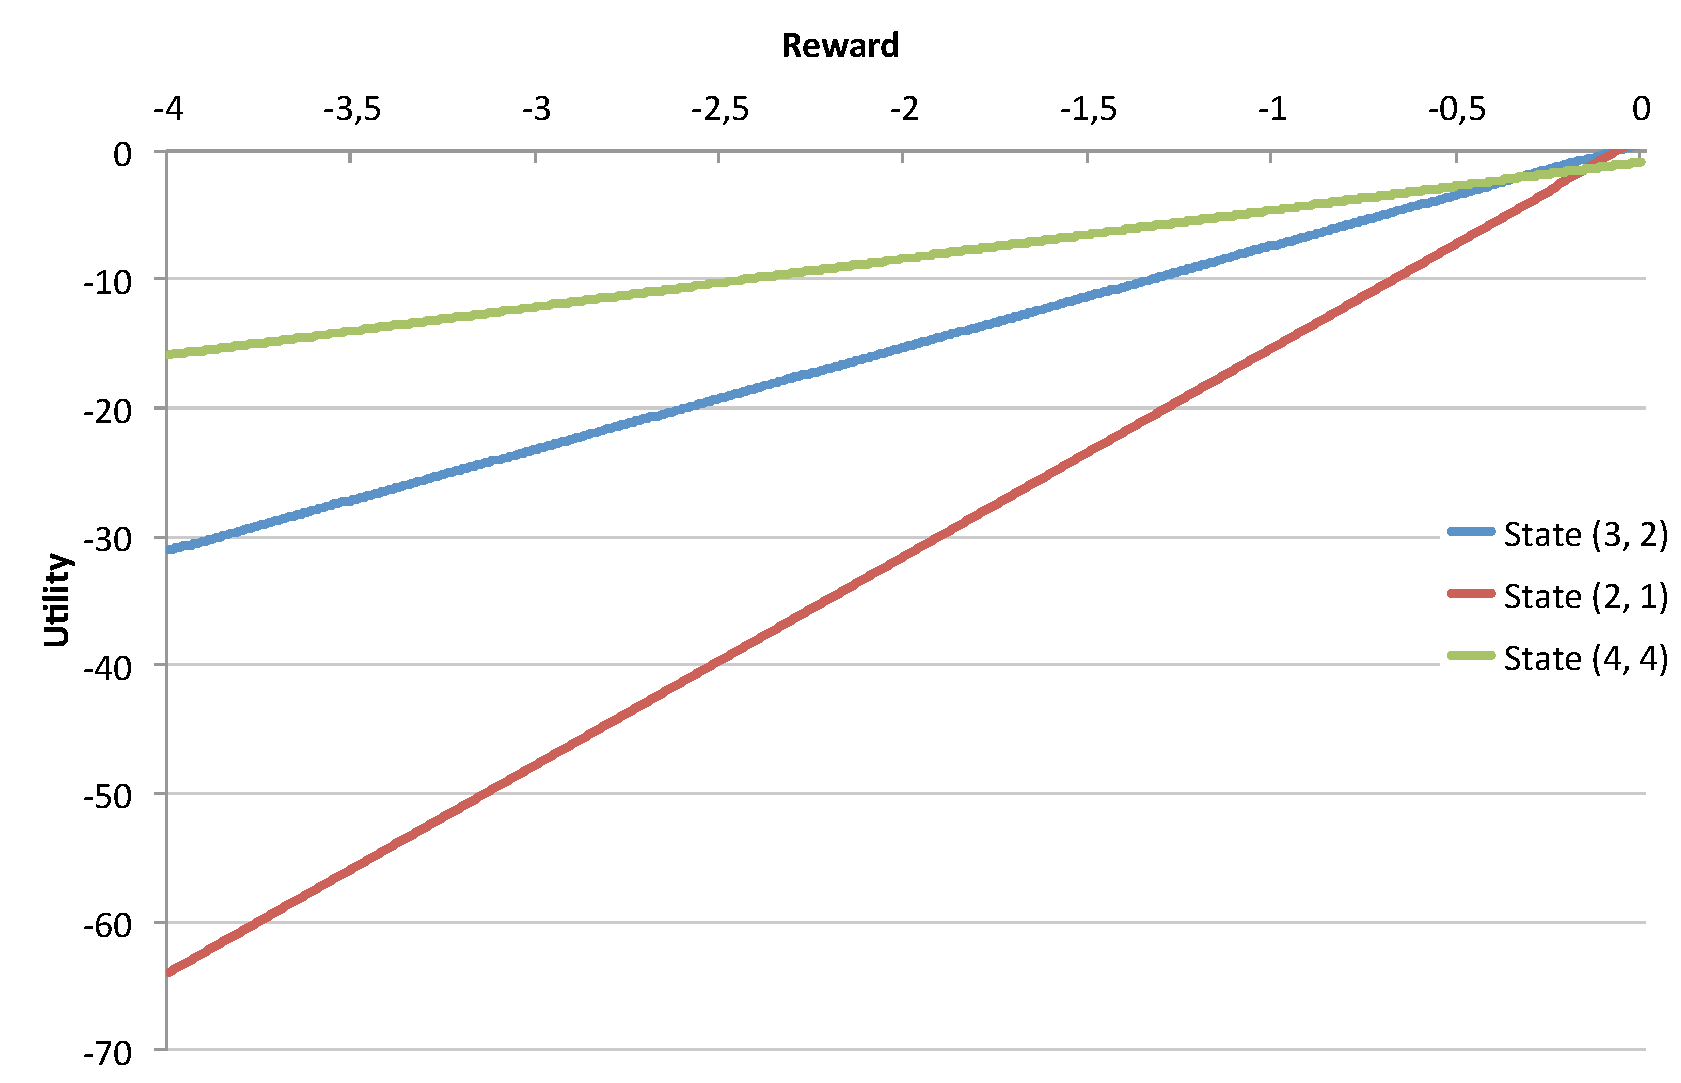
\includegraphics[width=\textwidth]{prob14}
	\caption{}
	\label{fig:prob14}
\end{figure}
\vfill

\clearpage

\subsection{From problem 1.5}
\label{ssec:prob15fig}
\vfill
\begin{figure}[h]
	\centering
	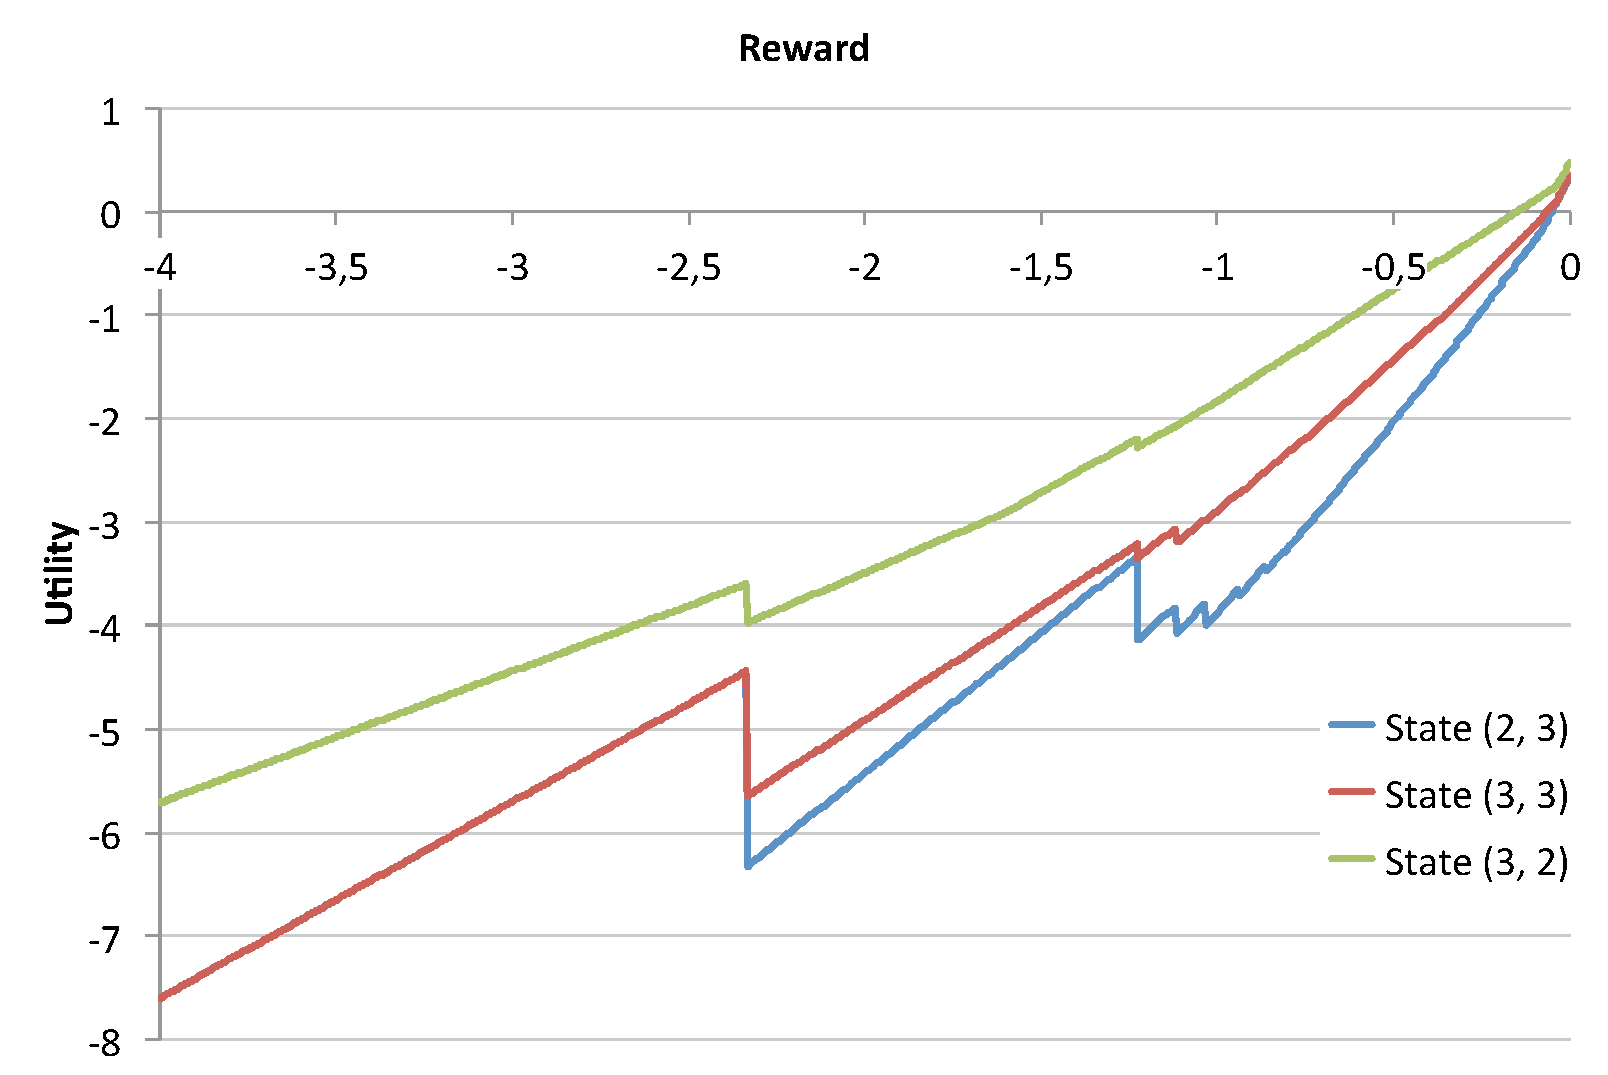
\includegraphics[width=\textwidth]{prob15}
	\caption{}
	\label{fig:prob15}
\end{figure}
\vfill
% (end)

\end{document}
